 
% easychair.tex,v 3.5 2017/03/15

\documentclass{easychair}
%\documentclass[EPiC]{easychair}
%\documentclass[EPiCempty]{easychair}
%\documentclass[debug]{easychair}
%\documentclass[verbose]{easychair}
%\documentclass[notimes]{easychair}
%\documentclass[withtimes]{easychair}
%\documentclass[a4paper]{easychair}
%\documentclass[letterpaper]{easychair}

\usepackage{xcolor}

\usepackage{doc}

\usepackage{cite}

% pretty tables defined with data files
\usepackage{booktabs}
\usepackage{longtable}
\usepackage{pgfplotstable}
\usepackage{titlesec}
\usepackage{multirow}
\usepackage{subcaption}
\usepackage{fancyvrb}
\usepackage{cleveref}

\pgfplotsset{compat=1.16}


% long table macro for pgfplotstable
% see https://tex.stackexchange.com/questions/66504/pgfplotstable-longtable-with-caption-and-repeating-header
\pgfkeysifdefined{/pgfplots/table/output empty row/.@cmd}{
    % upcoming releases offer this more convenient option:
    \pgfplotstableset{
        empty header/.style={
          every head row/.style={output empty row},
        }
    }
}{
    % versions up to and including 1.5.1 need this:
    \pgfplotstableset{
        empty header/.style={
            typeset cell/.append code={%
                \ifnum\pgfplotstablerow=-1 %
                    \pgfkeyssetvalue{/pgfplots/table/@cell content}{}%
                \fi
            }
        }
    }
}
%%%-----------------------------------------------

% use this if you have a long article and want to create an index
% \usepackage{makeidx}

% In order to save space or manage large tables or figures in a
% landcape-like text, you can use the rotating and pdflscape
% packages. Uncomment the desired from the below.
%
% \usepackage{rotating}
% \usepackage{pdflscape}

% Some of our commands for this guide.
%
\newcommand{\easychair}{\textsf{easychair}}
\newcommand{\miktex}{MiK{\TeX}}
\newcommand{\texniccenter}{{\TeX}nicCenter}
\newcommand{\makefile}{\texttt{Makefile}}
\newcommand{\latexeditor}{LEd}

\newcommand{\todoForParticipants}[1]{\textcolor{red}{TODO-PARTICIPANTS: #1}}

\newcommand{\todo}[1]{\textcolor{red}{TODO: #1}}

\titlespacing*{\paragraph}
{0pt}{2pt}{5pt}
%\makeindex

%% Front Matter
%%
% Regular title as in the article class.
%
\title{The Third International Verification of Neural Networks Competition (VNN-COMP 2022): Summary and Results%
%\thanks{Other people who contributed to this document include Maria Voronkov   (Imperial College and EasyChair) and Graham Gough (The University of Manchester).}
}

% Authors are joined by \and. Their affiliations are given by \inst, which indexes
% into the list defined using \institute
%
\author{Stanley Bak\thanks{S. Bak is with Stony Brook University, \tt stanley.bak@stonybrook.edu.}, Changliu Liu\thanks{C. Liu is with Carnegie Mellon University, \tt cliu6@andrew.cmu.edu.}, Taylor Johnson\thanks{T. Johnson is with Vanderbilt University, \tt taylor.johnson@vanderbilt.edu.}
%Serguei A. Mokhov\inst{1}\thanks{Designed and implemented the class style}
%\and
%    Geoff Sutcliffe\inst{2}\thanks{Did numerous tests and provided a lot of suggestions}
%\and
%   Andrei Voronkov\inst{3}\inst{4}\inst{5}\thanks{Masterminded EasyChair and created versions
%     3.0--3.5 of the class style}
}

% Institutes for affiliations are also joined by \and,
\institute{
%  Concordia University,
%  Montreal, Quebec, Canada\\
%  \email{mokhov@cse.concordia.ca}
%\and
%   University of Miami,
%   Miami, Florida, U.S.A.\\
%   \email{geoff@cs.miami.edu}\\
%\and
%   University of Manchester,
%   Manchester, U.K.\\
%   \email{andrei@voronkov.com}\\
%\and
%   Chalmers University of Technology,
%   Gothenburg, Sweden
%\and
%   EasyChair
 }

%  \authorrunning{} has to be set for the shorter version of the authors' names;
% otherwise a warning will be rendered in the running heads. When processed by
% EasyChair, this command is mandatory: a document without \authorrunning
% will be rejected by EasyChair

\authorrunning{}
\date{\phantom{date}\\}
% \titlerunning{} has to be set to either the main title or its shorter
% version for the running heads. When processed by
% EasyChair, this command is mandatory: a document without \titlerunning
% will be rejected by EasyChair
\titlerunning{VNN-COMP 2022 Report}

\begin{document}

\maketitle

\begin{abstract}
This report summarizes the third International Verification of Neural Networks Competition (VNN-COMP 2021), held as a part of the 5th Workshop on Formal Methods for ML-Enabled Autonomous Systems (FOMLAS) that was collocated with the 34th International Conference on Computer-Aided Verification (CAV).
%
%Twelve teams participated in this competition.
%
The goal of the competition is to provide an objective comparison of the state-of-the-art methods in neural network verification, in terms of scalability and speed.
%
Along this line, we used standard formats (ONNX for neural networks and VNNLIB for specifications), standard hardware (all tools are run by the organizers on AWS), and tool parameters provided by the tool authors.
%
This report summarizes the rules, benchmarks, participating tools, results, and lessons learned from this competition.
\end{abstract}



%------------------------------------------------------------------------------
%% Category carvana_unet_2022 (single_overhead=True):

\section{Total}

%Total Score:

\begin{table}[h]
\begin{center}
\caption{Overall Score} \label{tab:score}
{\setlength{\tabcolsep}{2pt}
\begin{tabular}[h]{@{}lll@{}}
\toprule
\textbf{\# ~} & \textbf{Tool} & \textbf{Score}\\
\midrule
1 & $\alpha$,$\beta$-CROWN & 1274.8 \\
2 & MN BaB & 980.6 \\
3 & Verinet & 893.8 \\
4 & Nnenum & 533.9 \\
5 & Cgdtest & 406.7 \\
6 & Peregrinn & 399.4 \\
7 & Marabou & 380.8 \\
8 & Debona & 222.9 \\
9 & Fastbatllnn & 100.0 \\
10 & Verapak & 98.3 \\
11 & Averinn & 29.1 \\
\bottomrule
\end{tabular}
}
\end{center}
\end{table}

\clearpage
\section{Scored}
% Category carvana_unet_2022 (single_overhead=True):

\begin{table}[h]
\begin{center}
\caption{Benchmark \texttt{carvana-unet-2022}} \label{tab:cat_{cat}}
{\setlength{\tabcolsep}{2pt}
\begin{tabular}[h]{@{}lllllrr@{}}
\toprule
\textbf{\# ~} & \textbf{Tool} & \textbf{Verified} & \textbf{Falsified} & \textbf{Fastest} & \textbf{Score} & \textbf{Percent}\\
\midrule
1 & $\alpha$,$\beta$-CROWN & 39 & 0 & 39 & 468 & 100.0\% \\
2 & MN BaB & 19 & 0 & 0 & 209 & 44.7\% \\
3 & Verinet & 3 & 0 & 0 & 30 & 6.4\% \\
\bottomrule
\end{tabular}
}
\end{center}
\end{table}



% Category cifar100_tinyimagenet_resnet (single_overhead=True):

\begin{table}[h]
\begin{center}
\caption{Benchmark \texttt{cifar100-tinyimagenet-resnet}} \label{tab:cat_{cat}}
{\setlength{\tabcolsep}{2pt}
\begin{tabular}[h]{@{}lllllrr@{}}
\toprule
\textbf{\# ~} & \textbf{Tool} & \textbf{Verified} & \textbf{Falsified} & \textbf{Fastest} & \textbf{Score} & \textbf{Percent}\\
\midrule
1 & $\alpha$,$\beta$-CROWN & 69 & 0 & 56 & 813 & 100.0\% \\
2 & Cgdtest & 95 & 0 & 28 & 725 & 89.2\% \\
3 & MN BaB & 60 & 3 & 10 & 674 & 82.9\% \\
4 & Verinet & 48 & 3 & 6 & 541 & 66.5\% \\
\bottomrule
\end{tabular}
}
\end{center}
\end{table}



% Category cifar_biasfield (single_overhead=True):

\begin{table}[h]
\begin{center}
\caption{Benchmark \texttt{cifar-biasfield}} \label{tab:cat_{cat}}
{\setlength{\tabcolsep}{2pt}
\begin{tabular}[h]{@{}lllllrr@{}}
\toprule
\textbf{\# ~} & \textbf{Tool} & \textbf{Verified} & \textbf{Falsified} & \textbf{Fastest} & \textbf{Score} & \textbf{Percent}\\
\midrule
1 & $\alpha$,$\beta$-CROWN & 69 & 1 & 1 & 735 & 100.0\% \\
2 & Cgdtest & 71 & 0 & 55 & 732 & 99.6\% \\
3 & Verinet & 69 & 1 & 0 & 721 & 98.1\% \\
4 & Verapak & 71 & 0 & 0 & 635 & 86.4\% \\
5 & MN BaB & 36 & 1 & 17 & 404 & 55.0\% \\
6 & Marabou & 27 & 0 & 0 & 270 & 36.7\% \\
7 & Nnenum & 4 & 0 & 0 & 43 & 5.9\% \\
\bottomrule
\end{tabular}
}
\end{center}
\end{table}



% Category collins_rul_cnn (single_overhead=True):

\begin{table}[h]
\begin{center}
\caption{Benchmark \texttt{collins-rul-cnn}} \label{tab:cat_{cat}}
{\setlength{\tabcolsep}{2pt}
\begin{tabular}[h]{@{}lllllrr@{}}
\toprule
\textbf{\# ~} & \textbf{Tool} & \textbf{Verified} & \textbf{Falsified} & \textbf{Fastest} & \textbf{Score} & \textbf{Percent}\\
\midrule
1 & Nnenum & 16 & 45 & 57 & 725 & 100.0\% \\
2 & MN BaB & 16 & 44 & 57 & 715 & 98.6\% \\
3 & $\alpha$,$\beta$-CROWN & 15 & 45 & 56 & 612 & 84.4\% \\
4 & Verinet & 16 & 43 & 0 & 590 & 81.4\% \\
5 & Peregrinn & 14 & 42 & 0 & 560 & 77.2\% \\
6 & Cgdtest & 1 & 42 & 43 & -984 & 0\% \\
\bottomrule
\end{tabular}
}
\end{center}
\end{table}



% Category mnist_fc (single_overhead=True):

\begin{table}[h]
\begin{center}
\caption{Benchmark \texttt{mnist-fc}} \label{tab:cat_{cat}}
{\setlength{\tabcolsep}{2pt}
\begin{tabular}[h]{@{}lllllrr@{}}
\toprule
\textbf{\# ~} & \textbf{Tool} & \textbf{Verified} & \textbf{Falsified} & \textbf{Fastest} & \textbf{Score} & \textbf{Percent}\\
\midrule
1 & $\alpha$,$\beta$-CROWN & 66 & 18 & 53 & 963 & 100.0\% \\
2 & Verinet & 53 & 18 & 50 & 817 & 84.8\% \\
3 & MN BaB & 53 & 18 & 47 & 804 & 83.5\% \\
4 & Debona & 48 & 18 & 38 & 737 & 76.5\% \\
5 & Nnenum & 48 & 11 & 29 & 648 & 67.3\% \\
6 & Marabou & 44 & 16 & 0 & 600 & 62.3\% \\
7 & Peregrinn & 27 & 11 & 7 & 394 & 40.9\% \\
8 & Cgdtest & 66 & 3 & 23 & 241 & 25.0\% \\
9 & Verapak & 40 & 2 & 42 & 104 & 10.8\% \\
\bottomrule
\end{tabular}
}
\end{center}
\end{table}



% Category nn4sys (single_overhead=True):

\begin{table}[h]
\begin{center}
\caption{Benchmark \texttt{nn4sys}} \label{tab:cat_{cat}}
{\setlength{\tabcolsep}{2pt}
\begin{tabular}[h]{@{}lllllrr@{}}
\toprule
\textbf{\# ~} & \textbf{Tool} & \textbf{Verified} & \textbf{Falsified} & \textbf{Fastest} & \textbf{Score} & \textbf{Percent}\\
\midrule
1 & $\alpha$,$\beta$-CROWN & 152 & 0 & 132 & 1791 & 100.0\% \\
2 & Verinet & 57 & 0 & 43 & 670 & 37.4\% \\
3 & MN BaB & 42 & 0 & 19 & 467 & 26.1\% \\
4 & Peregrinn & 24 & 0 & 22 & 284 & 15.9\% \\
5 & Nnenum & 23 & 0 & 8 & 246 & 13.7\% \\
6 & Debona & 2 & 0 & 2 & 24 & 1.3\% \\
7 & Cgdtest & 2 & 0 & 2 & -176 & 0\% \\
\bottomrule
\end{tabular}
}
\end{center}
\end{table}



% Category oval21 (single_overhead=True):

\begin{table}[h]
\begin{center}
\caption{Benchmark \texttt{oval21}} \label{tab:cat_{cat}}
{\setlength{\tabcolsep}{2pt}
\begin{tabular}[h]{@{}lllllrr@{}}
\toprule
\textbf{\# ~} & \textbf{Tool} & \textbf{Verified} & \textbf{Falsified} & \textbf{Fastest} & \textbf{Score} & \textbf{Percent}\\
\midrule
1 & $\alpha$,$\beta$-CROWN & 25 & 1 & 10 & 291 & 100.0\% \\
2 & MN BaB & 19 & 1 & 2 & 205 & 70.4\% \\
3 & Verinet & 17 & 1 & 1 & 189 & 64.9\% \\
4 & Marabou & 19 & 0 & 17 & 125 & 43.0\% \\
5 & Nnenum & 3 & 1 & 0 & 40 & 13.7\% \\
6 & Peregrinn & 1 & 0 & 0 & 10 & 3.4\% \\
7 & Cgdtest & 11 & 0 & 1 & -580 & 0\% \\
\bottomrule
\end{tabular}
}
\end{center}
\end{table}



% Category reach_prob_density (single_overhead=True):

\begin{table}[h]
\begin{center}
\caption{Benchmark \texttt{reach-prob-density}} \label{tab:cat_{cat}}
{\setlength{\tabcolsep}{2pt}
\begin{tabular}[h]{@{}lllllrr@{}}
\toprule
\textbf{\# ~} & \textbf{Tool} & \textbf{Verified} & \textbf{Falsified} & \textbf{Fastest} & \textbf{Score} & \textbf{Percent}\\
\midrule
1 & Nnenum & 22 & 14 & 21 & 410 & 100.0\% \\
2 & $\alpha$,$\beta$-CROWN & 22 & 14 & 23 & 406 & 99.0\% \\
3 & Verinet & 22 & 14 & 10 & 383 & 93.4\% \\
4 & MN BaB & 22 & 12 & 14 & 368 & 89.8\% \\
5 & Marabou & 17 & 14 & 12 & 334 & 81.5\% \\
6 & Peregrinn & 18 & 14 & 2 & 324 & 79.0\% \\
7 & Cgdtest & 0 & 5 & 5 & 60 & 14.6\% \\
8 & Debona & 0 & 2 & 2 & 24 & 5.9\% \\
\bottomrule
\end{tabular}
}
\end{center}
\end{table}



% Category rl_benchmarks (single_overhead=True):

\begin{table}[h]
\begin{center}
\caption{Benchmark \texttt{rl-benchmarks}} \label{tab:cat_{cat}}
{\setlength{\tabcolsep}{2pt}
\begin{tabular}[h]{@{}lllllrr@{}}
\toprule
\textbf{\# ~} & \textbf{Tool} & \textbf{Verified} & \textbf{Falsified} & \textbf{Fastest} & \textbf{Score} & \textbf{Percent}\\
\midrule
1 & $\alpha$,$\beta$-CROWN & 193 & 103 & 296 & 3552 & 100.0\% \\
2 & Verinet & 193 & 103 & 292 & 3547 & 99.9\% \\
3 & MN BaB & 193 & 103 & 288 & 3536 & 99.5\% \\
4 & Nnenum & 191 & 103 & 282 & 3504 & 98.6\% \\
5 & Peregrinn & 193 & 103 & 271 & 3502 & 98.6\% \\
6 & Marabou & 191 & 103 & 278 & 3496 & 98.4\% \\
7 & Debona & 153 & 99 & 240 & 3000 & 84.5\% \\
8 & Averinn & 92 & 8 & 16 & 1032 & 29.1\% \\
9 & Cgdtest & 10 & 24 & 29 & 98 & 2.8\% \\
10 & Verapak & 0 & 4 & 0 & 40 & 1.1\% \\
\bottomrule
\end{tabular}
}
\end{center}
\end{table}



% Category sri_resnet_a (single_overhead=True):

\begin{table}[h]
\begin{center}
\caption{Benchmark \texttt{sri-resnet-a}} \label{tab:cat_{cat}}
{\setlength{\tabcolsep}{2pt}
\begin{tabular}[h]{@{}lllllrr@{}}
\toprule
\textbf{\# ~} & \textbf{Tool} & \textbf{Verified} & \textbf{Falsified} & \textbf{Fastest} & \textbf{Score} & \textbf{Percent}\\
\midrule
1 & $\alpha$,$\beta$-CROWN & 20 & 12 & 7 & 356 & 100.0\% \\
2 & Cgdtest & 26 & 6 & 14 & 352 & 98.9\% \\
3 & MN BaB & 18 & 12 & 19 & 343 & 96.3\% \\
4 & Verinet & 12 & 12 & 4 & 248 & 69.7\% \\
5 & Marabou & 3 & 0 & 0 & 30 & 8.4\% \\
\bottomrule
\end{tabular}
}
\end{center}
\end{table}



% Category sri_resnet_b (single_overhead=True):

\begin{table}[h]
\begin{center}
\caption{Benchmark \texttt{sri-resnet-b}} \label{tab:cat_{cat}}
{\setlength{\tabcolsep}{2pt}
\begin{tabular}[h]{@{}lllllrr@{}}
\toprule
\textbf{\# ~} & \textbf{Tool} & \textbf{Verified} & \textbf{Falsified} & \textbf{Fastest} & \textbf{Score} & \textbf{Percent}\\
\midrule
1 & $\alpha$,$\beta$-CROWN & 28 & 11 & 8 & 432 & 100.0\% \\
2 & MN BaB & 27 & 11 & 24 & 431 & 99.8\% \\
3 & Cgdtest & 22 & 10 & 0 & 329 & 76.2\% \\
4 & Verinet & 20 & 11 & 4 & 319 & 73.8\% \\
5 & Marabou & 61 & 0 & 36 & -411 & 0\% \\
\bottomrule
\end{tabular}
}
\end{center}
\end{table}



% Category tllverifybench (single_overhead=True):

\begin{table}[h]
\begin{center}
\caption{Benchmark \texttt{tllverifybench}} \label{tab:cat_{cat}}
{\setlength{\tabcolsep}{2pt}
\begin{tabular}[h]{@{}lllllrr@{}}
\toprule
\textbf{\# ~} & \textbf{Tool} & \textbf{Verified} & \textbf{Falsified} & \textbf{Fastest} & \textbf{Score} & \textbf{Percent}\\
\midrule
1 & Fastbatllnn & 11 & 21 & 32 & 384 & 100.0\% \\
2 & MN BaB & 11 & 21 & 21 & 364 & 94.8\% \\
3 & $\alpha$,$\beta$-CROWN & 11 & 21 & 11 & 351 & 91.4\% \\
4 & Peregrinn & 10 & 21 & 7 & 324 & 84.4\% \\
5 & Verinet & 11 & 21 & 0 & 320 & 83.3\% \\
6 & Nnenum & 1 & 21 & 10 & 240 & 62.5\% \\
7 & Debona & 0 & 19 & 10 & 210 & 54.7\% \\
8 & Marabou & 4 & 15 & 2 & 194 & 50.5\% \\
9 & Cgdtest & 0 & 9 & 6 & 2 & 0.5\% \\
\bottomrule
\end{tabular}
}
\end{center}
\end{table}



% Category vggnet16_2022 (single_overhead=True):

\begin{table}[h]
\begin{center}
\caption{Benchmark \texttt{vggnet16-2022}} \label{tab:cat_{cat}}
{\setlength{\tabcolsep}{2pt}
\begin{tabular}[h]{@{}lllllrr@{}}
\toprule
\textbf{\# ~} & \textbf{Tool} & \textbf{Verified} & \textbf{Falsified} & \textbf{Fastest} & \textbf{Score} & \textbf{Percent}\\
\midrule
1 & $\alpha$,$\beta$-CROWN & 14 & 1 & 11 & 176 & 100.0\% \\
2 & Nnenum & 11 & 1 & 0 & 127 & 72.2\% \\
3 & MN BaB & 5 & 1 & 4 & 69 & 39.2\% \\
4 & Verinet & 5 & 1 & 0 & 60 & 34.1\% \\
5 & Cgdtest & 0 & 2 & 1 & -378 & 0\% \\
\bottomrule
\end{tabular}
}
\end{center}
\end{table}

\clearpage
\section{Unscored}

% Category acasxu (single_overhead=True):

\begin{table}[h]
\begin{center}
\caption{Benchmark \texttt{acasxu}} \label{tab:cat_{cat}}
{\setlength{\tabcolsep}{2pt}
\begin{tabular}[h]{@{}lllllrr@{}}
\toprule
\textbf{\# ~} & \textbf{Tool} & \textbf{Verified} & \textbf{Falsified} & \textbf{Fastest} & \textbf{Score} & \textbf{Percent}\\
\midrule
1 & Nnenum & 139 & 47 & 174 & 2218 & 100.0\% \\
2 & $\alpha$,$\beta$-CROWN & 139 & 43 & 56 & 1685 & 76.0\% \\
3 & Cgdtest & 85 & 30 & 115 & 680 & 30.7\% \\
\bottomrule
\end{tabular}
}
\end{center}
\end{table}


% Category cifar2020 (single_overhead=True):

\begin{table}[h]
\begin{center}
\caption{Benchmark \texttt{cifar2020}} \label{tab:cat_{cat}}
{\setlength{\tabcolsep}{2pt}
\begin{tabular}[h]{@{}lllllrr@{}}
\toprule
\textbf{\# ~} & \textbf{Tool} & \textbf{Verified} & \textbf{Falsified} & \textbf{Fastest} & \textbf{Score} & \textbf{Percent}\\
\midrule
1 & $\alpha$,$\beta$-CROWN & 148 & 38 & 176 & 1822 & 100.0\% \\
2 & MN BaB & 93 & 28 & 14 & 1313 & 72.1\% \\
3 & Nnenum & 66 & 19 & 0 & 850 & 46.7\% \\
4 & Cgdtest & 86 & 30 & 6 & 499 & 27.4\% \\
5 & Verapak & 0 & 15 & 0 & 150 & 8.2\% \\
6 & Verinet & 91 & 47 & 7 & -3868 & 0\% \\
7 & Marabou & 4 & 0 & 0 & -60 & 0\% \\
\bottomrule
\end{tabular}
}
\end{center}
\end{table}


\clearpage
\section{Stats}
%%%%%%%%%% Stats %%%%%%%%%%%


\section{Total Score}

%Total Score:

\begin{table}[h]
\begin{center}
\caption{Overall Score} \label{tab:score}
{\setlength{\tabcolsep}{2pt}
\begin{tabular}[h]{@{}lll@{}}
\toprule
\textbf{\# ~} & \textbf{Tool} & \textbf{Score}\\
\midrule
1 & $\alpha$,$\beta$-CROWN & 1274.9 \\
2 & MN BaB & 1017.3 \\
3 & Verinet & 892.5 \\
4 & Nnenum & 534.0 \\
5 & Cgdtest & 406.4 \\
6 & Peregrinn & 399.0 \\
7 & Marabou & 380.6 \\
8 & Debona & 222.9 \\
9 & Fastbatllnn & 100.0 \\
10 & Verapak & 98.2 \\
11 & Averinn & 29.1 \\
\bottomrule
\end{tabular}
}
\end{center}
\end{table}




\clearpage
\section{Scored Benchmarks}

% Category carvana_unet_2022 (single_overhead=True):

\begin{table}[h]
\begin{center}
\caption{Benchmark \texttt{carvana-unet-2022}} \label{tab:cat_{cat}}
{\setlength{\tabcolsep}{2pt}
\begin{tabular}[h]{@{}llllllrr@{}}
\toprule
\textbf{\# ~} & \textbf{Tool} & \textbf{Verified} & \textbf{Falsified} & \textbf{Fastest} & \textbf{Penalty} & \textbf{Score} & \textbf{Percent}\\
\midrule
1 & $\alpha$,$\beta$ Crown & 39 & 0 & 39 & 0 & 468 & 100.0\% \\
2 & MN BaB & 19 & 0 & 0 & 0 & 209 & 44.7\% \\
3 & Verinet & 3 & 0 & 0 & 0 & 30 & 6.4\% \\
\bottomrule
\end{tabular}
}
\end{center}
\end{table}



\begin{figure}[h]
\centerline{\includegraphics[width=\textwidth]{cactus/carvana_unet_2022.pdf}}
\caption{Cactus Plot for Carvana Unet 2022.}
\label{fig:quantPic}
\end{figure}


% Category cifar100_tinyimagenet_resnet (single_overhead=True):

\begin{table}[h]
\begin{center}
\caption{Benchmark \texttt{cifar100-tinyimagenet-resnet}} \label{tab:cat_{cat}}
{\setlength{\tabcolsep}{2pt}
\begin{tabular}[h]{@{}llllllrr@{}}
\toprule
\textbf{\# ~} & \textbf{Tool} & \textbf{Verified} & \textbf{Falsified} & \textbf{Fastest} & \textbf{Penalty} & \textbf{Score} & \textbf{Percent}\\
\midrule
1 & $\alpha$,$\beta$ Crown & 69 & 0 & 56 & 0 & 813 & 100.0\% \\
2 & Cgdtest & 95 & 0 & 28 & 3 & 725 & 89.2\% \\
3 & MN BaB & 60 & 3 & 10 & 0 & 674 & 82.9\% \\
4 & Verinet & 48 & 3 & 6 & 0 & 540 & 66.4\% \\
\bottomrule
\end{tabular}
}
\end{center}
\end{table}



\begin{figure}[h]
\centerline{\includegraphics[width=\textwidth]{cactus/cifar100_tinyimagenet_resnet.pdf}}
\caption{Cactus Plot for CIFAR100 Tiny ImageNet ResNet.}
\label{fig:quantPic}
\end{figure}


% Category cifar_biasfield (single_overhead=True):

\begin{table}[h]
\begin{center}
\caption{Benchmark \texttt{cifar-biasfield}} \label{tab:cat_{cat}}
{\setlength{\tabcolsep}{2pt}
\begin{tabular}[h]{@{}llllllrr@{}}
\toprule
\textbf{\# ~} & \textbf{Tool} & \textbf{Verified} & \textbf{Falsified} & \textbf{Fastest} & \textbf{Penalty} & \textbf{Score} & \textbf{Percent}\\
\midrule
1 & $\alpha$,$\beta$ Crown & 69 & 1 & 1 & 0 & 736 & 100.0\% \\
2 & Cgdtest & 71 & 0 & 55 & 1 & 731 & 99.3\% \\
3 & Verinet & 69 & 1 & 0 & 0 & 721 & 98.0\% \\
4 & Verapak & 71 & 0 & 0 & 1 & 635 & 86.3\% \\
5 & MN BaB & 36 & 1 & 17 & 0 & 404 & 54.9\% \\
6 & Marabou & 27 & 0 & 0 & 0 & 270 & 36.7\% \\
7 & Nnenum & 4 & 0 & 0 & 0 & 43 & 5.8\% \\
\bottomrule
\end{tabular}
}
\end{center}
\end{table}



\begin{figure}[h]
\centerline{\includegraphics[width=\textwidth]{cactus/cifar_biasfield.pdf}}
\caption{Cactus Plot for CIFAR Biasfield.}
\label{fig:quantPic}
\end{figure}


% Category collins_rul_cnn (single_overhead=True):

\begin{table}[h]
\begin{center}
\caption{Benchmark \texttt{collins-rul-cnn}} \label{tab:cat_{cat}}
{\setlength{\tabcolsep}{2pt}
\begin{tabular}[h]{@{}llllllrr@{}}
\toprule
\textbf{\# ~} & \textbf{Tool} & \textbf{Verified} & \textbf{Falsified} & \textbf{Fastest} & \textbf{Penalty} & \textbf{Score} & \textbf{Percent}\\
\midrule
1 & Nnenum & 16 & 45 & 58 & 0 & 727 & 100.0\% \\
2 & MN BaB & 16 & 44 & 57 & 0 & 715 & 98.3\% \\
3 & $\alpha$,$\beta$ Crown & 15 & 45 & 56 & 1 & 612 & 84.2\% \\
4 & Verinet & 16 & 43 & 0 & 0 & 590 & 81.2\% \\
5 & Peregrinn & 14 & 42 & 0 & 0 & 560 & 77.0\% \\
6 & Cgdtest & 1 & 42 & 43 & 15 & -984 & 0\% \\
\bottomrule
\end{tabular}
}
\end{center}
\end{table}



\begin{figure}[h]
\centerline{\includegraphics[width=\textwidth]{cactus/collins_rul_cnn.pdf}}
\caption{Cactus Plot for Collins Rul CNN.}
\label{fig:quantPic}
\end{figure}


% Category mnist_fc (single_overhead=True):

\begin{table}[h]
\begin{center}
\caption{Benchmark \texttt{mnist-fc}} \label{tab:cat_{cat}}
{\setlength{\tabcolsep}{2pt}
\begin{tabular}[h]{@{}llllllrr@{}}
\toprule
\textbf{\# ~} & \textbf{Tool} & \textbf{Verified} & \textbf{Falsified} & \textbf{Fastest} & \textbf{Penalty} & \textbf{Score} & \textbf{Percent}\\
\midrule
1 & $\alpha$,$\beta$ Crown & 66 & 18 & 53 & 0 & 963 & 100.0\% \\
2 & Verinet & 53 & 18 & 50 & 0 & 817 & 84.8\% \\
3 & MN BaB & 53 & 18 & 47 & 0 & 804 & 83.5\% \\
4 & Debona & 48 & 18 & 38 & 0 & 737 & 76.5\% \\
5 & Nnenum & 48 & 11 & 29 & 0 & 649 & 67.4\% \\
6 & Marabou & 44 & 16 & 0 & 0 & 600 & 62.3\% \\
7 & Peregrinn & 27 & 11 & 7 & 0 & 394 & 40.9\% \\
8 & Cgdtest & 66 & 3 & 23 & 5 & 241 & 25.0\% \\
9 & Verapak & 40 & 2 & 42 & 4 & 104 & 10.8\% \\
\bottomrule
\end{tabular}
}
\end{center}
\end{table}



\begin{figure}[h]
\centerline{\includegraphics[width=\textwidth]{cactus/mnist_fc.pdf}}
\caption{Cactus Plot for MNIST FC.}
\label{fig:quantPic}
\end{figure}


% Category nn4sys (single_overhead=True):

\begin{table}[h]
\begin{center}
\caption{Benchmark \texttt{nn4sys}} \label{tab:cat_{cat}}
{\setlength{\tabcolsep}{2pt}
\begin{tabular}[h]{@{}llllllrr@{}}
\toprule
\textbf{\# ~} & \textbf{Tool} & \textbf{Verified} & \textbf{Falsified} & \textbf{Fastest} & \textbf{Penalty} & \textbf{Score} & \textbf{Percent}\\
\midrule
1 & $\alpha$,$\beta$ Crown & 152 & 0 & 132 & 0 & 1799 & 100.0\% \\
2 & MN BaB & 106 & 0 & 8 & 0 & 1140 & 63.4\% \\
3 & Verinet & 57 & 0 & 43 & 0 & 661 & 36.7\% \\
4 & Peregrinn & 24 & 0 & 22 & 0 & 284 & 15.8\% \\
5 & Nnenum & 23 & 0 & 8 & 0 & 246 & 13.7\% \\
6 & Debona & 2 & 0 & 2 & 0 & 24 & 1.3\% \\
7 & Cgdtest & 2 & 0 & 2 & 2 & -176 & 0\% \\
\bottomrule
\end{tabular}
}
\end{center}
\end{table}



\begin{figure}[h]
\centerline{\includegraphics[width=\textwidth]{cactus/nn4sys.pdf}}
\caption{Cactus Plot for NN4SYS.}
\label{fig:quantPic}
\end{figure}


% Category oval21 (single_overhead=True):

\begin{table}[h]
\begin{center}
\caption{Benchmark \texttt{oval21}} \label{tab:cat_{cat}}
{\setlength{\tabcolsep}{2pt}
\begin{tabular}[h]{@{}llllllrr@{}}
\toprule
\textbf{\# ~} & \textbf{Tool} & \textbf{Verified} & \textbf{Falsified} & \textbf{Fastest} & \textbf{Penalty} & \textbf{Score} & \textbf{Percent}\\
\midrule
1 & $\alpha$,$\beta$ Crown & 25 & 1 & 10 & 0 & 291 & 100.0\% \\
2 & MN BaB & 19 & 1 & 2 & 0 & 205 & 70.4\% \\
3 & Verinet & 17 & 1 & 1 & 0 & 189 & 64.9\% \\
4 & Marabou & 19 & 0 & 17 & 1 & 125 & 43.0\% \\
5 & Nnenum & 3 & 1 & 0 & 0 & 40 & 13.7\% \\
6 & Peregrinn & 1 & 0 & 0 & 0 & 10 & 3.4\% \\
7 & Cgdtest & 11 & 0 & 1 & 7 & -580 & 0\% \\
\bottomrule
\end{tabular}
}
\end{center}
\end{table}



\begin{figure}[h]
\centerline{\includegraphics[width=\textwidth]{cactus/oval21.pdf}}
\caption{Cactus Plot for OVAL 21.}
\label{fig:quantPic}
\end{figure}


% Category reach_prob_density (single_overhead=True):

\begin{table}[h]
\begin{center}
\caption{Benchmark \texttt{reach-prob-density}} \label{tab:cat_{cat}}
{\setlength{\tabcolsep}{2pt}
\begin{tabular}[h]{@{}llllllrr@{}}
\toprule
\textbf{\# ~} & \textbf{Tool} & \textbf{Verified} & \textbf{Falsified} & \textbf{Fastest} & \textbf{Penalty} & \textbf{Score} & \textbf{Percent}\\
\midrule
1 & Nnenum & 22 & 14 & 22 & 0 & 411 & 100.0\% \\
2 & $\alpha$,$\beta$ Crown & 22 & 14 & 23 & 0 & 406 & 98.8\% \\
3 & Verinet & 22 & 14 & 10 & 0 & 383 & 93.2\% \\
4 & MN BaB & 22 & 12 & 14 & 0 & 368 & 89.5\% \\
5 & Marabou & 17 & 14 & 12 & 0 & 334 & 81.3\% \\
6 & Peregrinn & 18 & 14 & 2 & 0 & 324 & 78.8\% \\
7 & Cgdtest & 0 & 5 & 5 & 0 & 60 & 14.6\% \\
8 & Debona & 0 & 2 & 2 & 0 & 24 & 5.8\% \\
\bottomrule
\end{tabular}
}
\end{center}
\end{table}



\begin{figure}[h]
\centerline{\includegraphics[width=\textwidth]{cactus/reach_prob_density.pdf}}
\caption{Cactus Plot for Reachability Probability Density.}
\label{fig:quantPic}
\end{figure}


% Category rl_benchmarks (single_overhead=True):

\begin{table}[h]
\begin{center}
\caption{Benchmark \texttt{rl-benchmarks}} \label{tab:cat_{cat}}
{\setlength{\tabcolsep}{2pt}
\begin{tabular}[h]{@{}llllllrr@{}}
\toprule
\textbf{\# ~} & \textbf{Tool} & \textbf{Verified} & \textbf{Falsified} & \textbf{Fastest} & \textbf{Penalty} & \textbf{Score} & \textbf{Percent}\\
\midrule
1 & $\alpha$,$\beta$ Crown & 193 & 103 & 296 & 0 & 3552 & 100.0\% \\
2 & Verinet & 193 & 103 & 292 & 0 & 3547 & 99.9\% \\
3 & MN BaB & 193 & 103 & 288 & 0 & 3536 & 99.5\% \\
4 & Nnenum & 191 & 103 & 283 & 0 & 3506 & 98.7\% \\
5 & Peregrinn & 193 & 103 & 271 & 0 & 3502 & 98.6\% \\
6 & Marabou & 191 & 103 & 278 & 0 & 3496 & 98.4\% \\
7 & Debona & 153 & 99 & 240 & 0 & 3000 & 84.5\% \\
8 & Averinn & 92 & 8 & 16 & 0 & 1032 & 29.1\% \\
9 & Cgdtest & 10 & 24 & 29 & 3 & 98 & 2.8\% \\
10 & Verapak & 0 & 4 & 0 & 0 & 40 & 1.1\% \\
\bottomrule
\end{tabular}
}
\end{center}
\end{table}



\begin{figure}[h]
\centerline{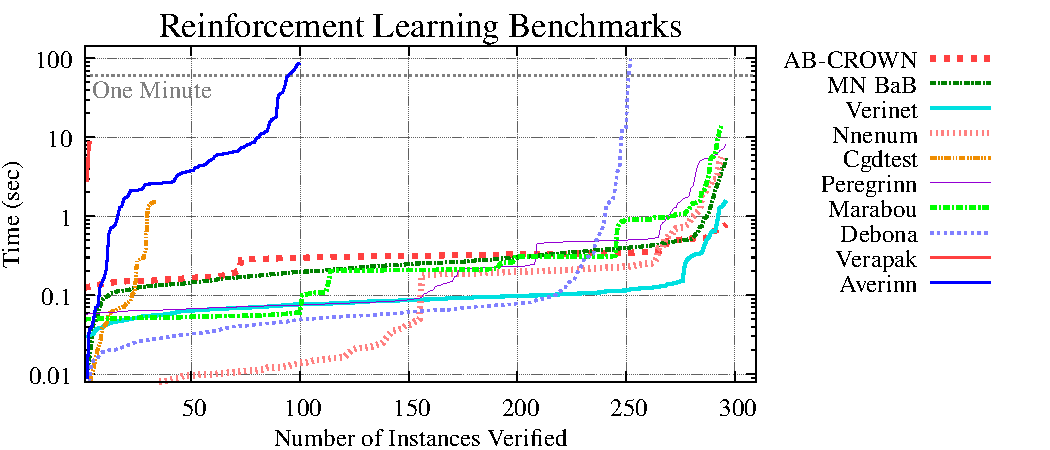
\includegraphics[width=\textwidth]{cactus/rl_benchmarks.pdf}}
\caption{Cactus Plot for Reinforcement Learning Benchmarks.}
\label{fig:quantPic}
\end{figure}


% Category sri_resnet_a (single_overhead=True):

\begin{table}[h]
\begin{center}
\caption{Benchmark \texttt{sri-resnet-a}} \label{tab:cat_{cat}}
{\setlength{\tabcolsep}{2pt}
\begin{tabular}[h]{@{}llllllrr@{}}
\toprule
\textbf{\# ~} & \textbf{Tool} & \textbf{Verified} & \textbf{Falsified} & \textbf{Fastest} & \textbf{Penalty} & \textbf{Score} & \textbf{Percent}\\
\midrule
1 & $\alpha$,$\beta$ Crown & 20 & 12 & 7 & 0 & 356 & 100.0\% \\
2 & Cgdtest & 26 & 6 & 14 & 0 & 352 & 98.9\% \\
3 & MN BaB & 18 & 12 & 19 & 0 & 343 & 96.3\% \\
4 & Verinet & 12 & 12 & 4 & 0 & 248 & 69.7\% \\
\bottomrule
\end{tabular}
}
\end{center}
\end{table}



\begin{figure}[h]
\centerline{\includegraphics[width=\textwidth]{cactus/sri_resnet_a.pdf}}
\caption{Cactus Plot for SRI Resnet A.}
\label{fig:quantPic}
\end{figure}


% Category sri_resnet_b (single_overhead=True):

\begin{table}[h]
\begin{center}
\caption{Benchmark \texttt{sri-resnet-b}} \label{tab:cat_{cat}}
{\setlength{\tabcolsep}{2pt}
\begin{tabular}[h]{@{}llllllrr@{}}
\toprule
\textbf{\# ~} & \textbf{Tool} & \textbf{Verified} & \textbf{Falsified} & \textbf{Fastest} & \textbf{Penalty} & \textbf{Score} & \textbf{Percent}\\
\midrule
1 & MN BaB & 27 & 11 & 24 & 0 & 435 & 100.0\% \\
2 & $\alpha$,$\beta$ Crown & 28 & 11 & 9 & 0 & 435 & 100.0\% \\
3 & Cgdtest & 22 & 10 & 9 & 0 & 340 & 78.2\% \\
4 & Verinet & 20 & 11 & 4 & 0 & 321 & 73.8\% \\
\bottomrule
\end{tabular}
}
\end{center}
\end{table}



\begin{figure}[h]
\centerline{\includegraphics[width=\textwidth]{cactus/sri_resnet_b.pdf}}
\caption{Cactus Plot for SRI Resnet B.}
\label{fig:quantPic}
\end{figure}


% Category tllverifybench (single_overhead=True):

\begin{table}[h]
\begin{center}
\caption{Benchmark \texttt{tllverifybench}} \label{tab:cat_{cat}}
{\setlength{\tabcolsep}{2pt}
\begin{tabular}[h]{@{}llllllrr@{}}
\toprule
\textbf{\# ~} & \textbf{Tool} & \textbf{Verified} & \textbf{Falsified} & \textbf{Fastest} & \textbf{Penalty} & \textbf{Score} & \textbf{Percent}\\
\midrule
1 & Fastbatllnn & 11 & 21 & 32 & 0 & 384 & 100.0\% \\
2 & MN BaB & 11 & 21 & 21 & 0 & 364 & 94.8\% \\
3 & $\alpha$,$\beta$ Crown & 11 & 21 & 12 & 0 & 353 & 91.9\% \\
4 & Peregrinn & 10 & 21 & 7 & 0 & 324 & 84.4\% \\
5 & Verinet & 11 & 21 & 0 & 0 & 320 & 83.3\% \\
6 & Nnenum & 1 & 21 & 10 & 0 & 240 & 62.5\% \\
7 & Debona & 0 & 19 & 10 & 0 & 210 & 54.7\% \\
8 & Marabou & 4 & 15 & 2 & 0 & 194 & 50.5\% \\
9 & Cgdtest & 0 & 9 & 6 & 1 & 2 & 0.5\% \\
\bottomrule
\end{tabular}
}
\end{center}
\end{table}



\begin{figure}[h]
\centerline{\includegraphics[width=\textwidth]{cactus/tllverifybench.pdf}}
\caption{Cactus Plot for Two-Level Lattice Verify Benchmark.}
\label{fig:quantPic}
\end{figure}


% Category vggnet16_2022 (single_overhead=True):

\begin{table}[h]
\begin{center}
\caption{Benchmark \texttt{vggnet16-2022}} \label{tab:cat_{cat}}
{\setlength{\tabcolsep}{2pt}
\begin{tabular}[h]{@{}llllllrr@{}}
\toprule
\textbf{\# ~} & \textbf{Tool} & \textbf{Verified} & \textbf{Falsified} & \textbf{Fastest} & \textbf{Penalty} & \textbf{Score} & \textbf{Percent}\\
\midrule
1 & $\alpha$,$\beta$ Crown & 14 & 1 & 11 & 0 & 176 & 100.0\% \\
2 & Nnenum & 11 & 1 & 0 & 0 & 127 & 72.2\% \\
3 & MN BaB & 5 & 1 & 4 & 0 & 69 & 39.2\% \\
4 & Verinet & 5 & 1 & 0 & 0 & 60 & 34.1\% \\
5 & Cgdtest & 0 & 2 & 1 & 4 & -378 & 0\% \\
\bottomrule
\end{tabular}
}
\end{center}
\end{table}



\begin{figure}[h]
\centerline{\includegraphics[width=\textwidth]{cactus/vggnet16_2022.pdf}}
\caption{Cactus Plot for VGGNet16 2022.}
\label{fig:quantPic}
\end{figure}



\clearpage
\section{Unscored Benchmarks}

% Category acasxu (single_overhead=True):

\begin{table}[h]
\begin{center}
\caption{Benchmark \texttt{acasxu}} \label{tab:cat_{cat}}
{\setlength{\tabcolsep}{2pt}
\begin{tabular}[h]{@{}llllllrr@{}}
\toprule
\textbf{\# ~} & \textbf{Tool} & \textbf{Verified} & \textbf{Falsified} & \textbf{Fastest} & \textbf{Penalty} & \textbf{Score} & \textbf{Percent}\\
\midrule
1 & Nnenum & 139 & 47 & 174 & 0 & 2218 & 100.0\% \\
2 & $\alpha$,$\beta$-CROWN & 139 & 46 & 59 & 0 & 2021 & 91.1\% \\
3 & MN BaB & 110 & 46 & 52 & 0 & 1664 & 75.0\% \\
4 & Cgdtest & 85 & 30 & 115 & 7 & 680 & 30.7\% \\
\bottomrule
\end{tabular}
}
\end{center}
\end{table}



% Category cifar2020 (single_overhead=True):

\begin{table}[h]
\begin{center}
\caption{Benchmark \texttt{cifar2020}} \label{tab:cat_{cat}}
{\setlength{\tabcolsep}{2pt}
\begin{tabular}[h]{@{}llllllrr@{}}
\toprule
\textbf{\# ~} & \textbf{Tool} & \textbf{Verified} & \textbf{Falsified} & \textbf{Fastest} & \textbf{Penalty} & \textbf{Score} & \textbf{Percent}\\
\midrule
1 & Verinet & 91 & 35 & 109 & 0 & 1486 & 100.0\% \\
2 & $\alpha$,$\beta$-CROWN & 95 & 34 & 78 & 0 & 1479 & 99.5\% \\
3 & MN BaB & 93 & 28 & 26 & 0 & 1275 & 85.8\% \\
4 & Nnenum & 66 & 19 & 0 & 0 & 850 & 57.2\% \\
5 & Cgdtest & 63 & 26 & 5 & 6 & 305 & 20.5\% \\
6 & Verapak & 0 & 15 & 1 & 0 & 152 & 10.2\% \\
7 & Marabou & 4 & 0 & 0 & 1 & -60 & 0\% \\
\bottomrule
\end{tabular}
}
\end{center}
\end{table}




\clearpage
\section{Stats}

%%%%%%%%%% Stats %%%%%%%%%%%

% Overhead:

\begin{table}[h]
\begin{center}
\caption{Overhead} \label{tab:overhead}
{\setlength{\tabcolsep}{2pt}
\begin{tabular}[h]{@{}llr@{}}
\toprule
\textbf{\# ~} & \textbf{Tool} & \textbf{Seconds}\\
\midrule
1 & Marabou & 0.2 \\
2 & Fastbatllnn & 0.5 \\
3 & Nnenum & 0.9 \\
4 & Cgdtest & 1.3 \\
5 & Peregrinn & 1.3 \\
6 & Debona & 2.0 \\
7 & Averinn & 3.1 \\
8 & Verinet & 3.4 \\
9 & Verapak & 4.6 \\
10 & $\alpha$,$\beta$ Crown & 6.7 \\
11 & MN BaB & 8.2 \\
\bottomrule
\end{tabular}
}
\end{center}
\end{table}



% Num Benchmarks Participated:

\begin{table}[h]
\begin{center}
\caption{Num Benchmarks Participated} \label{tab:stats0}
{\setlength{\tabcolsep}{2pt}
\begin{tabular}[h]{@{}llr@{}}
\toprule
\textbf{\# ~} & \textbf{Tool} & \textbf{Count}\\
\midrule
1 & Verinet & 13 \\
2 & MN BaB & 13 \\
3 & $\alpha$,$\beta$ Crown & 13 \\
4 & Cgdtest & 12 \\
5 & Nnenum & 9 \\
6 & Peregrinn & 7 \\
7 & Marabou & 6 \\
8 & Debona & 5 \\
9 & Verapak & 3 \\
10 & Fastbatllnn & 1 \\
11 & Averinn & 1 \\
\bottomrule
\end{tabular}
}
\end{center}
\end{table}



% Num Instances Verified:

\begin{table}[h]
\begin{center}
\caption{Num Instances Verified} \label{tab:stats1}
{\setlength{\tabcolsep}{2pt}
\begin{tabular}[h]{@{}llr@{}}
\toprule
\textbf{\# ~} & \textbf{Tool} & \textbf{Count}\\
\midrule
1 & $\alpha$,$\beta$ Crown & 950 \\
2 & MN BaB & 812 \\
3 & Verinet & 754 \\
4 & Nnenum & 515 \\
5 & Peregrinn & 478 \\
6 & Marabou & 450 \\
7 & Cgdtest & 405 \\
8 & Debona & 341 \\
9 & Verapak & 117 \\
10 & Averinn & 100 \\
11 & Fastbatllnn & 32 \\
\bottomrule
\end{tabular}
}
\end{center}
\end{table}



% Num SAT:

\begin{table}[h]
\begin{center}
\caption{Num SAT} \label{tab:stats2}
{\setlength{\tabcolsep}{2pt}
\begin{tabular}[h]{@{}llr@{}}
\toprule
\textbf{\# ~} & \textbf{Tool} & \textbf{Count}\\
\midrule
1 & Verinet & 228 \\
2 & MN BaB & 227 \\
3 & $\alpha$,$\beta$ Crown & 227 \\
4 & Nnenum & 196 \\
5 & Peregrinn & 191 \\
6 & Marabou & 148 \\
7 & Debona & 138 \\
8 & Cgdtest & 101 \\
9 & Fastbatllnn & 21 \\
10 & Averinn & 8 \\
11 & Verapak & 6 \\
\bottomrule
\end{tabular}
}
\end{center}
\end{table}



% Num UNSAT:

\begin{table}[h]
\begin{center}
\caption{Num UNSAT} \label{tab:stats3}
{\setlength{\tabcolsep}{2pt}
\begin{tabular}[h]{@{}llr@{}}
\toprule
\textbf{\# ~} & \textbf{Tool} & \textbf{Count}\\
\midrule
1 & $\alpha$,$\beta$ Crown & 723 \\
2 & MN BaB & 585 \\
3 & Verinet & 526 \\
4 & Nnenum & 319 \\
5 & Cgdtest & 304 \\
6 & Marabou & 302 \\
7 & Peregrinn & 287 \\
8 & Debona & 203 \\
9 & Verapak & 111 \\
10 & Averinn & 92 \\
11 & Fastbatllnn & 11 \\
\bottomrule
\end{tabular}
}
\end{center}
\end{table}



% Incorrect Results (or Missing CE):

\begin{table}[h]
\begin{center}
\caption{Incorrect Results (or Missing CE)} \label{tab:stats4}
{\setlength{\tabcolsep}{2pt}
\begin{tabular}[h]{@{}llr@{}}
\toprule
\textbf{\# ~} & \textbf{Tool} & \textbf{Count}\\
\midrule
1 & Cgdtest & 41 \\
2 & Verapak & 5 \\
3 & Marabou & 1 \\
4 & $\alpha$,$\beta$ Crown & 1 \\
\bottomrule
\end{tabular}
}
\end{center}
\end{table}




%\input{introduction}

%\input{rules}

%\input{participants}

%\input{benchmarks}

%\input{results}

%\input{conclusion}

%\input{acks}

%\label{sect:bib}

%\bibliographystyle{plain}
%\bibliographystyle{alpha}
%\bibliographystyle{unsrt}
%\bibliographystyle{abbrv}
%\bibliography{bib/nnv,bib/nnenum,bib/peregriNN,bib/verinet,bib/oval,bib/venus,bib/MIPVerify, bib/ERAN, bib/alpha-beta-CROWN,bib/debona,bib/dnnf,bib/nvjl,bib/nn4sys,bib/Marabou,bib/RPM}


%------------------------------------------------------------------------------

%------------------------------------------------------------------------------
% Index
%\printindex

%------------------------------------------------------------------------------
\end{document}

